\documentclass[12pt]{article}
\usepackage[paper=letterpaper,margin=1.5cm]{geometry}
\usepackage{amsmath,amssymb,amsfonts}
\usepackage{newtxtext, newtxmath}
\usepackage{graphicx}
\usepackage{physics}
\usepackage{enumitem}
\usepackage{titling}
\usepackage[colorlinks=true]{hyperref}
\usepackage{autobreak}
\usepackage{listings}
\usepackage[font=small,labelfont=bf]{caption} % Required for specifying captions to tables and figures

\usepackage{graphicx} % Required for the inclusion of images
\graphicspath{{./images/}} % Specifies the directory where pictures are stored

\setlength{\droptitle}{-6em}
\begin{document}

\center
Aprendizagem 2024\\
Homework III -- Group 016\\
(ist1106022, ist1106720)\vskip 1cm

\large{\textbf{Part I}: Pen and paper}\normalsize
\begin{enumerate}[leftmargin=\labelsep, label=\textbf{\arabic*.)}]
    \item \begin{itemize}
              \item Dataset Provided:
                    \[\begin{array}{|c|c|c|c|c|}
                            \hline
                            x   & y_1 & y_2 & y_{\text{num}} & y_{\text{class}} \\
                            \hline
                            x_1 & 1   & 1   & 1.25           & B                \\
                            x_2 & 1   & 3   & 7.0            & A                \\
                            x_3 & 3   & 2   & 2.7            & C                \\
                            x_4 & 3   & 3   & 3.2            & A                \\
                            x_5 & 2   & 4   & 5.5            & B                \\
                            \hline
                        \end{array}\]
                    \vspace{0.5em}
              \item Transformed Features for each Observation \\
                    \vspace{0.5em}
                    \begin{minipage}{1\textwidth}
                        \begin{center}
                            \[\begin{array}{|c|c|c|c|c}
                                    \hline
                                    x   & y_1 & y_2 & \phi(y_1, y_2) \\
                                    \hline
                                    x_1 & 1   & 1   & 1 \times 1 = 1 \\
                                    x_2 & 1   & 3   & 1 \times 3 = 3 \\
                                    x_3 & 3   & 2   & 3 \times 2 = 6 \\
                                    x_4 & 3   & 3   & 3 \times 3 = 9 \\
                                    x_5 & 2   & 4   & 2 \times 4 = 8 \\
                                    \hline
                                \end{array}\]
                        \end{center}
                    \end{minipage}
                    \vspace{0.5em}
              \item OLS Closed-Form Solution \\
                    \vspace{0.5em}
                    The Ordinary Least Squares (OLS) closed-form solution is given by:
                    \[
                        w = ({X}^T {X})^{-1} {X}^T z
                    \]
                    Where, in this case, X is the matrix of the transformed features $\phi(y_1, y_2)$ and z is the vector of targeted values $y_{\text{num}}$.
                    \vspace{0.5em}
              \item Desgin Matrix \\
                    We add a column of 1's to represent the intercept term in linear regression:
                    \[
                        X = \begin{bmatrix} 1 & 1 \\ 1 & 3 \\ 1 & 6 \\ 1 & 9 \\ 1 & 8 \end{bmatrix}
                    \]
              \item Target Vector \\
                    The target vector $y_{\text{num}}$ is:
                    \[
                        z = \begin{bmatrix} 1.25 \\ 7.0 \\ 2.7 \\ 3.2 \\ 5.5 \end{bmatrix}
                    \]
              \item OLS Coefficient Calculations \\
                    \vspace{0.5em}
                    \begin{minipage}{1\textwidth}
                        \[
                            w = (\begin{bmatrix} 1 & 1 & 1 & 1 & 1 \\ 1 & 3 & 6 & 9 & 8 \end{bmatrix} \begin{bmatrix} 1 & 1 \\ 1 & 3 \\ 1 & 6 \\ 1 & 9 \\ 1 & 8 \end{bmatrix})^{-1} \begin{bmatrix} 1 & 1 & 1 & 1 & 1 \\ 1 & 3 & 6 & 9 & 8 \end{bmatrix} \begin{bmatrix} 1.25 \\ 7.0 \\ 2.7 \\ 3.2 \\ 5.5 \end{bmatrix}
                        \]
                        \[
                            w = (\begin{bmatrix} 5 & 27 \\ 27 & 191 \end{bmatrix})^{-1} \begin{bmatrix} 19.65 \\ 111.25 \end{bmatrix}
                        \]
                        \[
                            w = \frac{1}{5 \times 191 - 27 \times 27} \begin{bmatrix} 191 & -27 \\ -27 & 5 \end{bmatrix} \begin{bmatrix} 19.65 \\ 111.25 \end{bmatrix}
                        \]
                        \[
                            w = \begin{bmatrix} 3.31593 \\ 0.113717 \end{bmatrix}
                        \]

                        Thus, the estimated regression coefficients are:
                        \[
                            w_{\text{0}} = 3.31593
                        \]
                        \[
                            w_{\text{1}} = 0.11372
                        \]

                    \end{minipage}
                    \vspace{0.5em}
              \item Learned Regression Model:
                    \[
                        y_{\text{num}} = 3.31593 + 0.11372 \times (y_1 \times y_2)
                    \]
                    This model can be used to predict the continuous output \( y_{\text{num}} \) based on new input values \( y_1 \) and \( y_2 \).
          \end{itemize}
          \vspace{0.5em}
    \item \begin{itemize}
              \item Ridge Closed-Form Solution \\
                    \vspace{0.5em}
                    The Ridge closed-form solution is given by:
                    \[
                        w = ({X}^T {X} + \lambda I)^{-1} {X}^T z
                    \]
                    Where, in this case:
                    \begin{itemize}
                        \item X is the design matrix (same as the one in OLS),
                        \item z is the target vector (same as the one in OLS),
                        \item \( \lambda = 1 \) is the regularization parameter,
                        \item \( I \) is the identity matrix (same size as ${X}^T{X}$).
                    \end{itemize}
                    \vspace{0.5em}
              \item Ridge Coefficient Calculations \\
                    \vspace{0.5em}
                    \begin{minipage}{1\textwidth}
                        \[
                            w = (\begin{bmatrix} 1 & 1 & 1 & 1 & 1 \\ 1 & 3 & 6 & 9 & 8 \end{bmatrix} \begin{bmatrix} 1 & 1 \\ 1 & 3 \\ 1 & 6 \\ 1 & 9 \\ 1 & 8 \end{bmatrix} + 1 \times \begin{bmatrix} 1 & 0 \\ 0 & 1 \end{bmatrix})^{-1} \begin{bmatrix} 1 & 1 & 1 & 1 & 1 \\ 1 & 3 & 6 & 9 & 8 \end{bmatrix} \begin{bmatrix} 1.25 \\ 7.0 \\ 2.7 \\ 3.2 \\ 5.5 \end{bmatrix}
                        \]
                        \[
                            w = (\begin{bmatrix} 5 & 27 \\ 27 & 191 \end{bmatrix} + \begin{bmatrix} 1 & 0 \\ 0 & 1 \end{bmatrix})^{-1} \begin{bmatrix} 19.65 \\ 111.25 \end{bmatrix}
                        \]
                        \[
                            w = (\begin{bmatrix} 6 & 27 \\ 27 & 192 \end{bmatrix})^{-1} \begin{bmatrix} 19.65 \\ 111.25 \end{bmatrix}
                        \]
                        \[
                            w = \frac{1}{6 \times 192 - 27 \times 27} \begin{bmatrix} 192 & -27 \\ -27 & 6 \end{bmatrix} \begin{bmatrix} 19.65 \\ 111.25 \end{bmatrix}
                        \]
                        \[
                            w = \begin{bmatrix} 1.81809 \\ 0.323759 \end{bmatrix}
                        \]

                        Thus, the estimated regression coefficients are:
                        \[
                            w_{\text{0}} = 1.81809
                        \]
                        \[
                            w_{\text{1}} = 0.32376
                        \]

                    \end{minipage}
                    \vspace{0.5em}
              \item Learned Regression Model:
                    \[
                        y_{\text{num}} = 1.81809 + 0.32376 \times (y_1 \times y_2)
                    \]
                    This model can be used to predict the continuous output \( y_{\text{num}} \) based on new input values \( y_1 \) and \( y_2 \).
                    \vspace{0.5em}
              \item Coefficients and Regularization: \\
                    The Ridge Regression coefficient is smaller than the OLS coefficient. This is due to the regularization term $\lambda$, which penalizes large coefficient values. Regularization helps to control overfitting by making the model less sensitive to small fluctuations in the data.

          \end{itemize}

    \item \begin{itemize}
              \item RMSE Formula \\
                    \vspace{0.5em}
                    The formula for RMSE is:
                    \[
                        \text{RMSE} = \sqrt{\frac{1}{n} \sum_{i=1}^{n} (z_i - \hat{z}_i)^2}
                    \]
                    Where:
                    \begin{itemize}
                        \item \( z_i \) are the actual values,
                        \item \( \hat{z}_i \) are the predicted values,
                        \item \( n \) is the number of observations.
                    \end{itemize}
                    \vspace{0.5em}
              \item The new test data provided is: \\
                    \[
                        \begin{array}{|c|c|c|c|}
                            \hline
                            \text{Test Observation} & y_1 & y_2 & y_{\text{num}} \\
                            \hline
                            x_6                     & 2   & 2   & 0.7            \\
                            x_7                     & 1   & 2   & 1.1            \\
                            x_8                     & 5   & 1   & 2.2            \\
                            \hline
                        \end{array}
                    \]

                    Using the basis function \( \phi(y_1, y_2) = y_1 \times y_2 \), the transformed features for the test set are:
                    \[
                        \Phi_{\text{test}} = \begin{bmatrix} 4 \\ 2 \\ 5 \end{bmatrix}
                    \]

              \item Predictions for Train and Test Sets \\

                    We use the learned regression models from both the OLS and Ridge models to predict \( y_{\text{num}} \) for both the train and test sets.

                    - OLS Learned Regression: \( y_{\text{num}} = 3.31593 + 0.11372 \times (y_1 \times y_2) \) \\
                    - Ridge Learned Regresion: \( y_{\text{num}} = 1.81809 + 0.32376 \times (y_1 \times y_2) \)

                    \[
                        X_{\text{train}} = \begin{bmatrix} 1 & 1 \\ 1 & 3 \\ 1 & 6 \\ 1 & 9 \\ 1 & 8 \end{bmatrix}
                    \]

                    \[
                        X_{\text{test}} = \begin{bmatrix} 1 & 4 \\ 1 & 2 \\ 1 & 5 \end{bmatrix}
                    \]

                    The predicted values for the train set using the OLS and Ridge models are:
                    \[
                        \hat{Y}_{\text{train, OLS}} = X_{\text{train}} \times \hat{w}_{\text{OLS}} = \begin{bmatrix} 1 & 1 \\ 1 & 3 \\ 1 & 6 \\ 1 & 9 \\ 1 & 8 \end{bmatrix} \times \begin{bmatrix} 3.31593 \\ 0.11372 \end{bmatrix} = \begin{bmatrix} 3.42965 \\ 3.65709 \\ 3.99825 \\ 4.33941 \\ 4.22569 \end{bmatrix}
                    \]
                    \[
                        \hat{Y}_{\text{train, Ridge}} = X_{\text{train}} \times \hat{w}_{\text{ridge}} = \begin{bmatrix} 1 & 1 \\ 1 & 3 \\ 1 & 6 \\ 1 & 9 \\ 1 & 8 \end{bmatrix} \times \begin{bmatrix} 1.81809 \\ 0.32376 \end{bmatrix} = \begin{bmatrix} 2.14185 \\ 2.78937 \\ 3.76065 \\ 4.73193 \\ 4.40817 \end{bmatrix}
                    \]

                    For the test set, the predicted values are:
                    \[
                        \hat{Y}_{\text{test, OLS}} = X_{\text{test}} \times \hat{w}_{\text{OLS}} = \begin{bmatrix} 1 & 4 \\ 1 & 2 \\ 1 & 5 \end{bmatrix} \times \begin{bmatrix} 3.31593 \\ 0.11372 \end{bmatrix} = \begin{bmatrix} 3.77081 \\ 3.54337 \\ 3.88453 \end{bmatrix}
                    \]
                    \[
                        \hat{Y}_{\text{test, Ridge}} = X_{\text{test}} \times \hat{w}_{\text{ridge}} = \begin{bmatrix} 1 & 4 \\ 1 & 2 \\ 1 & 5 \end{bmatrix} \times \begin{bmatrix} 1.81809 \\ 0.32376 \end{bmatrix} = \begin{bmatrix} 3.11313 \\ 2.46561 \\ 3.43689 \end{bmatrix}
                    \]

              \item RMSE Calculation

                    To calculate RMSE, we use the formula for both the train and test sets.

                    For the train set:

                    \scalebox{0.8}{$
                        \text{RMSE}_{\text{train, OLS}} = \sqrt{\frac{1}{5} \left( (1.25 - 3.42965)^2 + (7.0 - 3.65709)^2 + (2.7 - 3.99825)^2 + (3.2 - 4.33941)^2 + (5.5 - 4.22569)^2 \right)} = 2.0265
                    $}

                    \scalebox{0.8}{$
                        \text{RMSE}_{\text{train, Ridge}} = \sqrt{\frac{1}{5} \left( (1.25 - 2.14185)^2 + (7.0 - 2.78937)^2 + (2.7 - 3.76065)^2 + (3.2 - 4.73193)^2 + (5.5 - 4.40817)^2 \right)} = 2.15354
                    $}

                    For the test set:

                    \[
                        \text{RMSE}_{\text{test, OLS}} = \sqrt{\frac{1}{3} \left( (0.7 - 3.77081)^2 + (1.1 - 3.54337)^2 + (2.2 - 3.88453)^2 \right)} = 2.46560
                    \]
                    \[
                        \text{RMSE}_{\text{test, Ridge}} = \sqrt{\frac{1}{3} \left( (0.7 - 3.11313)^2 + (1.1 - 2.46561)^2 + (2.2 - 3.43689)^2 \right)} = 1.75290
                    \]

              \item Conclusion

                    \[
                        \begin{array}{|c|c|c|}
                            \hline
                            \text{Model} & \text{Train RMSE} & \text{Test RMSE} \\
                            \hline
                            OLS          & 2.0265            & 2.46560          \\
                            Ridge        & 2.15354           & 1.75290          \\
                            \hline
                        \end{array}
                    \]

                    \vspace{0.75em}
                    The OLS Model achieves a lower RMSE on the training set, which may lead to overfitting. In contrast, it shows a higher RMSE on the test set, which indicates poor generalization to new data due to overfitting. These results are as expected, since OLS does not regularize the model and tends to perform worse on new data. \\
                    \vspace{1em}
                    The Ridge Model achieves a higher RMSE on the training set, as regularization sacrificies some accuracy. In contrast, it shows a lower RMSE on the test set, which indicates better generalization to new data compared to the OLS Model. These results are as expected, since the Ridge regression's regularization helps prevent overfitting, making it more reliable for new data.

          \end{itemize}
    \item To perform a stochastic gradient descent update on the weights and bias, we must first perform a foward propagation to calculate the output of the model, and then a backward propagation to calculate the gradients of the loss functions and use them to update the weights and bias.
          \begin{itemize}
              \item \textbf{Initial Assumptions:} Besides everything already stated in the question:
                    \begin{center}

                        \vspace{0.25cm}

                        $z = \begin{bmatrix}
                                0 \\
                                1 \\
                                0
                            \end{bmatrix}$, since the $y_\text{class}$ for $x_1$ is B

                        \vspace{0.25cm}
                    \end{center}
              \item \textbf{Forward Propagation:}
                    \begin{center}

                        \vspace{0.25cm}
                        $Z^{[1]}= W^{[1]}X^{[0]} + b^{[1]}$  \hspace{2em}
                        $Z^{[1]}= \begin{bmatrix}
                                0,1 & 0,1 \\
                                0,1 & 0,2 \\
                                0,2 & 0,1
                            \end{bmatrix} \cdot \begin{bmatrix}
                                1 \\
                                1
                            \end{bmatrix} + \begin{bmatrix}
                                0,1 \\
                                0   \\
                                0,1
                            \end{bmatrix} = \begin{bmatrix}
                                0,3 \\
                                0,3 \\
                                0,4
                            \end{bmatrix}$
                        \vspace{0.5em}

                        $X^{[1]} = Z^{[1]}$ (no activation function)
                        \vspace{0.5em}

                        $Z^{[2]}= W^{[2]}X^{[1]} + b^{[2]}$  \hspace{2em}
                        $Z^{[2]}= \begin{bmatrix}
                                1 & 2 & 2 \\
                                1 & 2 & 1 \\
                                1 & 1 & 1
                            \end{bmatrix} \cdot \begin{bmatrix}
                                0,3 \\
                                0,3 \\
                                0,4
                            \end{bmatrix} + \begin{bmatrix}
                                1 \\
                                1 \\
                                1
                            \end{bmatrix} = \begin{bmatrix}
                                2,7 \\
                                2,3 \\
                                2
                            \end{bmatrix}$
                        \vspace{0.5em}

                        $X^{[2]} = \text{softmax}(Z^{[2]}) = \begin{bmatrix}
                                \frac{e^{2,7}}{e^{2,7} + e^{2,3} + e^2} \\
                                \frac{e^{2,3}}{e^{2,7} + e^{2,3} + e^2} \\
                                \frac{e^2}{e^{2,7} + e^{2,3} + e^2}
                            \end{bmatrix} = \begin{bmatrix}
                                0,46149 \\
                                0,30934 \\
                                0,22918
                            \end{bmatrix}$
                        \vspace{0.25cm}
                    \end{center}
              \item \textbf{Backward Propagation:}
                    \begin{center}
                        \vspace{0.25cm}
                        Considering that the loss function is the cross-entropy loss, the gradients are calculated as follows:
                        $$\pdv{E}{W^{[P]}} = (\pdv{E}{X^{[P]}} \circ \pdv{X^{[P]}}{Z^{[P]}}) \cdot \pdv{Z^{[P]}}{W^{[P]}} = \delta^{[P]} \cdot (X^{[P-1]})^{T}$$

                        For the output layer we have:
                        \vspace{0.5em}

                        $\delta^{[P]} = (X^{[N]} - Z)$ \hspace{2em}
                        $\delta^{[2]} = (X^{[2]} - Z) = \begin{bmatrix}
                                0,46149 \\
                                0,30934 \\
                                0,22918
                            \end{bmatrix} - \begin{bmatrix}
                                0 \\
                                1 \\
                                0
                            \end{bmatrix} = \begin{bmatrix}
                                0,46149  \\
                                -0,69066 \\
                                0,22918
                            \end{bmatrix}$

                        \vspace{0.5em}

                        $\pdv{E}{W^{[2]}} = \delta^{[2]} \cdot (X^{[1]})^{T} = \begin{bmatrix}
                                0,46149  \\
                                -0,69066 \\
                                0,22918
                            \end{bmatrix} \cdot \begin{bmatrix}
                                0,3 & 0,3 & 0,4
                            \end{bmatrix} = \begin{bmatrix}
                                0,13845  & 0,13845  & 0,18460  \\
                                -0,20720 & -0,20720 & -0,27626 \\
                                0,06876  & 0,06876  & 0,09167
                            \end{bmatrix}$
                        \vspace{0.25cm}

                        For the hidden layer we have:
                        \vspace{0.5em}

                        $\delta^{[P]} = (W^{[P+1]})^{T} \cdot \delta^{[P+1]} \circ \phi^{\prime[P]}(Z^{[P]})$ \hspace{2em}
                        $\delta^{[1]} = (W^{[2]})^{T} \cdot \delta^{[2]} \circ \phi^{\prime[1]}(Z^{[1]})$
                        \vspace{0.5em}

                        Since the hidden layer has no activation function, $\phi^{\prime[1]}(Z^{[1]}) = 1$:
                        \vspace{0.5em}

                        $\delta^{[1]} = (W^{[2]})^{T} \cdot \delta^{[2]} = \begin{bmatrix}
                                1 & 1 & 1 \\
                                2 & 2 & 1 \\
                                2 & 1 & 1
                            \end{bmatrix} \cdot \begin{bmatrix}
                                0,46149  \\
                                -0,69066 \\
                                0,22918
                            \end{bmatrix} = \begin{bmatrix}
                                0        \\
                                -0,22916 \\
                                0,46150
                            \end{bmatrix}$
                        \vspace{0.5em}

                        $\pdv{E}{W^{[1]}} = \delta^{[1]} \cdot (X^{[0]})^{T} = \begin{bmatrix}
                                0        \\
                                -0,22916 \\
                                0,46150
                            \end{bmatrix} \cdot \begin{bmatrix}
                                1 \\
                                1
                            \end{bmatrix} = \begin{bmatrix}
                                0        & 0        \\
                                -0,22916 & -0,22916 \\
                                0,46150  & 0,46150
                            \end{bmatrix}$

                    \end{center}
              \item \textbf{Weight Update:}
                    \begin{center}
                        \vspace{0.25cm}

                        $W^{[P]} = W^{[P]} - \eta \pdv{E}{W^{[P]}}$
                        \vspace{0.5em}

                        $W^{[2]} = W^{[2]} - \eta \pdv{E}{W^{[2]}} = \begin{bmatrix}
                                1 & 2 & 2 \\
                                1 & 2 & 1 \\
                                1 & 1 & 1
                            \end{bmatrix} - 0,1 \cdot \begin{bmatrix}
                                0,13845  & 0,13845  & 0,18460  \\
                                -0,20720 & -0,20720 & -0,27626 \\
                                0,06876  & 0,06876  & 0,09167
                            \end{bmatrix} = \ \begin{bmatrix}
                                0,98616 & 1,98616 & 1,98154 \\
                                1,02072 & 2,02072 & 1,02763 \\
                                0,99312 & 0,99312 & 0,99083
                            \end{bmatrix}$

                        \vspace{0.25cm}

                        $W^{[1]} = W^{[1]} - \eta \pdv{E}{W^{[1]}} = \begin{bmatrix}
                                0,1 & 0,1 \\
                                0,1 & 0,2 \\
                                0,2 & 0,1
                            \end{bmatrix} - 0,1 \cdot \begin{bmatrix}
                                0        & 0        \\
                                -0,22916 & -0,22916 \\
                                0,46150  & 0,46150
                            \end{bmatrix} = \begin{bmatrix}
                                0,1     & 0,1     \\
                                0,12292 & 0,22292 \\
                                0,15385 & 0,05385
                            \end{bmatrix}$
                        \vspace{0.25cm}

                    \end{center}
              \item \textbf{Bias Update:}
                    \begin{center}
                        \vspace{0.25cm}

                        $b^{[P]} = b^{[P]} - \eta \pdv{E}{b^{[P]}} = b^{[P]} - \eta \delta^{[P]}$ (since $\pdv{E}{b^{[P]}} = \delta^{[P]}$)

                        \vspace{0.5em}

                        $b^{[2]} = b^{[2]} - \eta \delta^{[2]} = \begin{bmatrix}
                                1 \\
                                1 \\
                                1
                            \end{bmatrix} - 0,1 \cdot \begin{bmatrix}
                                0,46149  \\
                                -0,69066 \\
                                0,22918
                            \end{bmatrix} = \begin{bmatrix}
                                0,95385 \\
                                1,06907 \\
                                0,97708
                            \end{bmatrix}$

                        $b^{[1]} = b^{[1]} - \eta \delta^{[1]} = \begin{bmatrix}
                                0,1 \\
                                0   \\
                                0,1
                            \end{bmatrix} - 0,1 \cdot \begin{bmatrix}
                                0        \\
                                -0,22916 \\
                                0,46150
                            \end{bmatrix} = \begin{bmatrix}
                                0,1     \\
                                0,02292 \\
                                0,05385
                            \end{bmatrix}$



                        \vspace{0.25cm}
                    \end{center}
          \end{itemize}
\end{enumerate}


\large{\textbf{Part II}: Programming}\normalsize
\begin{enumerate}[leftmargin=\labelsep, label=\textbf{\arabic*.)},start=5]
    \item To compare the performance of a Linear Regression Model and two MLP Regressors with 2 hidden layers of 10 neurons each, except one has no activation function while the other has ReLU activation functions, we averaged out the performance of each model over 10 separate runs on different 80-20 train-test splits. The resulting boxplots for each model are:

          \begin{center}
              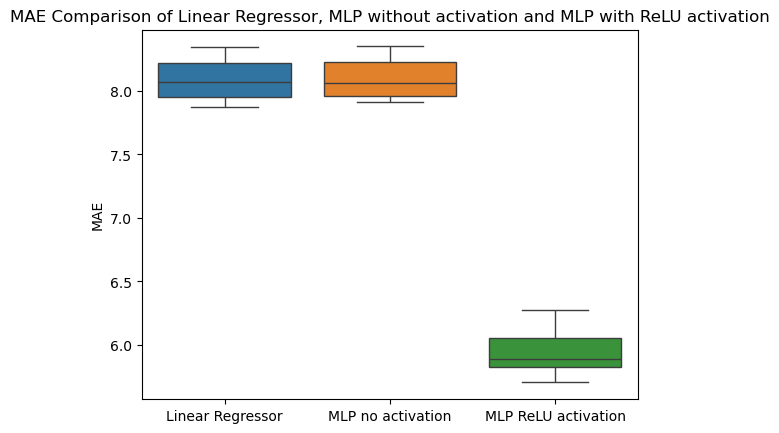
\includegraphics[width=0.8\textwidth]{boxplot_models_MAE.png}
              \captionof{figure}{Boxplot graphs for the Mean Absolute Error of different regression models, accross 80-20 train-test splits.}
          \end{center}

    \item As expected the Linear and MLP without activation regressors have high similar absolute errors, since they can only be used in linearly separable datasets. By adding an activation function, such as ReLU, on the MLP model we are able to learn non-linear patterns within the dataset, which obviously results in a lower absolute error.

          The reason that no activation function, which in reality is the default sign function, leads to bad results is because it creates a linear decision boundary, which is not suitable for non-linear datasets, that can't be separated by simple lines, but rather complex non-linear boundaries.

    \item MLP regressors have varied hyperparameters that can be tuned to improve their performance. To find the best combination of hyperparameters, within the choices presented in the assignment, we used a grid search approach, with a single split, applied on all combinations. The results were as follows:

          \begin{center}
              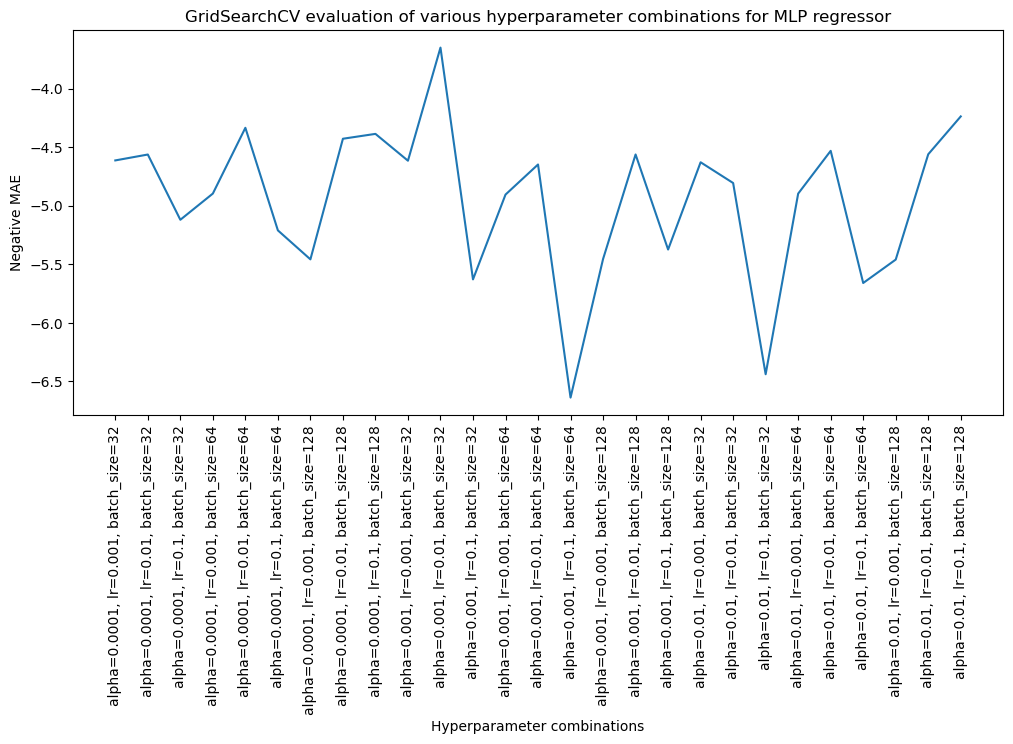
\includegraphics[width=0.8\textwidth]{hyperparameters_performance_plot.png}
              \captionof{figure}{Performance of different hyperparameters combinations on the MLP Regressor}
          \end{center}

          As it can be seen on the plot, the best L2 penalty - Learning Rate - Batch size combination is the one that leads to the lowest Mean Absolute Error, which is the following combination:

          \begin{itemize}
              \item L2 penalty: 0.001
              \item Learning Rate: 0.01
              \item Batch Size: 32
          \end{itemize}

          All of these parameters have a varied impact on the performance of a MLP regressor:
          \begin{itemize}
              \item \textbf{L2 penalty:} Regularization term applied on the loss function. It prevents overfitting by penalizing large weight fluctuations. It encourages small changes in the weights, which lead to reduced complexity and better generalization. However, if the penalty is too high, important patterns in the data may be lost and the bias increases. As such, the chosen penalty of 0.001 is the middle choice between the given options, that balances the trade-off in fitting and complexity.
              \item \textbf{Learning Rate:} Determines the step size in the gradient descent optimization process. A small learning rate can help the model converge to a minimum optimal point, although it may require more iterations and sometimes get stuck on a local minimum, while a big learning rate can overshoot the optimal point. Therefore, as seen in the plot, a smaller learning rate of 0.01 is the most optimal of the given choices.
              \item \textbf{Batch Size:} Determines the number of observation samples used in each iteration for training, essentially how many how many samples will be propagated through the neural network to give an output and then update the weights. Smaller batch sizes require less memory and can speed up training, but are more sensible to noisy data and therefore lead to less accurate gradients. On the opossite end, larger batch sizes lead to more accurate gradients, but require more memory and are slower to train. In this case, a batch size of 32 was the most optimal of the given choices (the other parameters also influenced this decision, if batch size were the sole factor, a larger batch size would be better).
          \end{itemize}
\end{enumerate}
\end{document}
